\documentclass[10pt,a4paper,final]{report}
\usepackage[utf8]{inputenc}
\usepackage{amsmath}
\usepackage{amsfonts}
\usepackage{listings}
\usepackage{amssymb}
\usepackage{graphicx}
\usepackage[utf8]{inputenc}
\usepackage[english]{babel}
\begin{document}

\newtheorem{theorem}{Teorema}
\newtheorem{proof}{Proof}
%TODO ver como arreglar esto de proof
\newtheorem{lemma}{Lema}
\newtheorem{definition}{Definición}
\newtheorem{proposition}{Proposition}
\newtheorem{observation}{Observation}
\newtheorem{corollary}{Corollary}
\newtheorem{example}{Examples}

\section{Punto flotante y redondeo}
{
	Sea $x=0,a_1 a_2...a_m... 10^l$. Es decir, x está en el rango de la máquina (podría no estarlo y en ese caso no podríamos aproximarlo bien).
	
Hay dos formas de aproximar a $x$. Una es por truncamiento y la otra por redondeo.

¿Cómo es el error absoluto, y el relativo en cada paso?

\begin{itemize}
	\item Truncamiento: $|x-x^*| = 0,0...0a_{m+1}a_{m+2}... 10^l \geq 10^{l-m}$ porque los $a_j$ podrían ser todos 9.
	\item Redondeo: $|x-x^*| \geq 0,0...05 10^l = \frac{1}{2} 10^{l-m}$. Esta cuenta también se puede hacer contando la cantidad de números de máquina entre $10^{l-1}$ y $10^{l}$, que están uniformemente distribuidos. Son $9 10^{m-1}$. La distancia entre $x$ y $x*$ va a ser menor o igual a la mitad de la distancia entre dos números de máquina en $[10^{l-1}, 10^{l}]$ porque siempre se toma el más cercano, es decir, $\frac{9 10^{l-1}}{2 9 10^{m-1}} = \frac{1}{2} 10^{l-m}$, como queríamos ver.
\end{itemize}
}



\section{Métodos iterativos para resolver sistemas lineales}

Primero, una cuenta explicando cómo es Gauss-Seidel.

La idea de Jacobi era despejar la coordenada iésima del nuevo vector a partir de la iésima ecuación. La idea de Gauss Seidel es aprovechar los cálculos hechos hasta ahora.

Luego definimos $x_i^{k+1}=\frac{b_i - \sum_{j=1}^{i-1}a_{ij}x_j^{k+1}-\sum_{j=1}^{i-1}a_{ij}x_j^{k}}{a_{ii}}$\\

Si pasamos multiplicando $a_ii$ y sumando la primer sumatoria, obtenemos la siguiente igualdad:

$a_{ii} x_i^{k+1} + \sum_{j=1}^{i-1}a_{ij}x_j^{k+1} =  b_i - \sum_{j=1}^{i-1} a_{ij} x_j^{k}$\\

Juntando, obtenemos lo siguiente:

$\sum_{j=1}^{i}a_{ij}x_j^{k+1} =  b_i - \sum_{j=1}^{i-1} a_{ij} x_j^{k}$\\

Expresemos esto en forma matricial:

$(L+D) x^{k+1} = b - U x_k$. O sea:\\

$x^{k+1} = - (L+D)^{-1} U x_k + (L+D)^{-1} b$\\

Es decir, obtuvimos que $B_{GS} = - (L+D)^{-1} U$. Fantástico.

-----------------------------


\begin{definition}Una matriz A se dice estrictamente diagonal dominante si $|a_{ii}| > \sum_{j\neq i} |a_{ij}|$
\end{definition}

\begin{theorem}Si A es estrictamente diagonal dominante, ambos métodos convergentes
\end{theorem}

\begin{proof}
\textbf{Jacobi}: basta ver que $||B_J||_{\infty}<1$

Recordemos que $B_J = -D^{-1}(L+U)$, es decir,\\

$b_{ij}=-\frac{a{ij}}{a_{ii}}$ para $i\neq j$ y $b_{ii}=0$

Luego $||B_J||_{\infty} = \underset{i}{max} \frac{\sum_{j\neq i} |a_{ij}|}{|a_{ii}|}<1$ pues $A$ es diagonal dominante. \bigskip

\textbf{Gauss-Seidel} Este es un poquito más triqui, y vamos a necesitar probar que $\rho(B)<1$.

$B_{GS} = - (L+D)^{-1} U$

Sea $||x||_\infty=1$ autovector de autovalor $\lambda$. Luego $- (L+D)^{-1} Ux = \lambda x$. Como no sé manejar bien inversas, la paso para el otro lado, quedando:

$-Ux = \lambda (L+D) x$

Es decir, para cada $i$ tenemos $- \sum_{j=i+1}^N a_{ij} x_j = \lambda \sum_{j=1}^i a_{ij} x_j$

Ahora bien, yo quiero acotar $\lambda$ por 1 usando que la matriz es diagonal dominante. Necesito que aparezcan solas tanto $\lambda$ como $a_ii$.

La igualdad de arriba se puede expresar también como $- \sum_{j=i+1}^N a_{ij} x_j = \lambda \sum_{j=1}^{i-1} a_{ij} x_j + \lambda a_{ii} x_i$. Es decir:\\

$\lambda a_{ii} x_i = - \sum_{j=i+1}^N a_{ij} x_j -  \lambda \sum_{j=1}^{i-1} a_{ij} x_j$

Como quiero acotar $\lambda$, no paso sumando el último término sino que primero meto módulo. Como quiero deshacerme de $x_i$ pido $i$ tal que $x_i$ realice la norma infinito. (Por lo tanto $|x_j|\leq |x_i|$ y también puedo deshacerme de ellos). Queda:

$|\lambda| |a_{ii}| \leq \sum_{j=i+1}^N |a_{ij}| + \lambda \sum_{j=1}^{i-1} |a_{ij}|$. Ahora si paso restando para juntar los lambda:

$|\lambda| |a_{ii}| -  \lambda \sum_{j=1}^{i-1} |a_{ij}|\leq \sum_{j=i+1}^N |a_{ij}|$\\

$|\lambda| (|a_{ii}| - \sum_{j=1}^{i-1} |a_{ij}|)\leq \sum_{j=i+1}^N |a_{ij}|$\\

$|\lambda| \leq \frac{\sum_{j=i+1}^N |a_{ij}|}{(|a_{ii}| - \sum_{j=1}^{i-1} |a_{ij}|)}<1$ pues A es estrictamente diagonal dominante\\

\end{proof}
-------------------

%TODO me falta hacer bien la inducción en la descomposición de Cholesky

%TODO me faltan la descomposición de House Holder y la QR

\subsection{Método de House Holder}

Queremos escribir $A=QR$, porque si queremos resolver $Ax = b$ esto es lo mismo que $QRx = b$ y podemos multiplicar por $Q^t$ a ambos lados para obtener $Rx = Q^t b$

La idea es buscar una $Q$ ortonormal tal que $Qa_1 = (\pm ||x||,0,...,0)^t$, donde $a_1$ es la primer columna de $A$, y luego hacer inducción.

Vamos a reflejar.

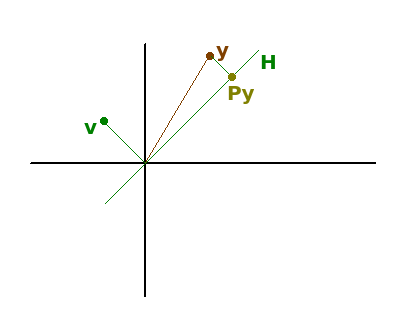
\includegraphics[scale=1]{householder1.png}

Tenemos que $y=P_y + <y,v> v$ entonces, despejando, resulta $P_y = y-v<v,y>$. Luego la proyección está dada por $P=Id-vv^t$.

Sea $||w||=1$. Entonces definimos $Q=Id-2ww^t$. El $2$ sale de que queremos reflejar. Es fácil chequear que $Q$ es ortogonal: $Q^t Q = (Id - 2 w w^t) (Id - 2 w w^t)$ pues $w w^t$ es simétrica.

Entonces $Q^t Q = Id - 4 w w^t + 4 w w^t w w^t$, pero $w^t w=||w||^2 = 1$ luego $Q^t Q = Id$, como queríamos ver. ¿Por qué queríamos ver esto? Porque queremos construirnos una $Q$ ortogonal tal que $Qa_1 = (\pm ||x||,0,...,0)^t$

Si en lugar de $w$ de norma 1 empezamos con un $v$ cualquiera, uno se da cuenta de que para que $Q$ sea ortogonal necesitamos definirla como $Q = Id - 2 \frac{v v^t}{v^t v}$. Una buena pregunta sería por qué esto sigue siendo una reflexión. Debe ser equivalente a la reflexión tomando $w=\frac{v}{||v||}$, probar esto.

Llamos $x=a_1$ para eliminar el subíndice.

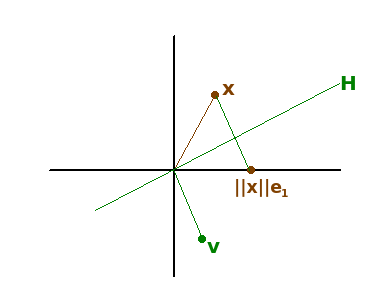
\includegraphics[scale=1]{householder2.png}

El $v$ que debemos usar para que la reflexión caiga en $||x||e_1$ es justamente $v_1=||x||e_1 - x$, y $Q_1 = Id - 2 \frac{v_1 v_1^t}{v_1^t v_1}$

Una observación es que podríamos haber tomado $\hat{v} = - ||x||e_1 -x$ y también habría funcionado. En general, como no quiero restar cosas parecidas para que no haya cancelaciones catastróficas, voy a tomar $v= -sg(x_1)||x||e_1-x$.

\subsection*{Gram-Schmidt}

\begin{observation}
	Algo interesante es que también podemos obtener las matrices $Q$ y $R$ haciendo Gram-Schmidt. Si llamo $a_j$ a las columnas de $A$, la idea es que $Q$ sea los vectores obtenidos durante la ortonormalización de $A$.
	
	Definimos $R = Q^t A = (Q_i^t a_j)$. Observemos que si $i>j$ entonces $a_j$ es combinación lineal de $Q_1,...,Q_j$; por lo tanto $Q_i^t a_j = 0$. Luego $R$ es efectivamente triangular superior.
	
Ah, pero ¿quién dice que $QR = A$? ¡Esto hay que probarlo! $R = Q^t A \Rightarrow Q R = Q Q^t A = Id A = A$. Uff, qué susto.

Última observación: ¿Qué pasa si $A \in \mathbb{R}^{m\times n}$, con $m>n$? O sea, tiene más filas que columnas.

Gram-Schmidt puedo hacer alegremente, y también definir $R= Q^t A$.

Pero ojo, no es cierto que $QQ^t = Id$

(continuará)

\end{observation}



%TODO escribirlo transpuesto

\begin{theorem}

 Si $A$ es simétrica y definida positiva entonces GS converge, pero Jacobi puede no converger (no fue demostrado)
\end{theorem}
--------------------------

\begin{proposition}Si $B=-M^{-1}N$ entonces $\lambda$ autovalor de $B$ si y solo si $det(\lambda M + N) = 0$
\end{proposition}

\begin{proof}

$det(\lambda Id - B) = 0 \Leftrightarrow det(\lambda Id + M^{-1}N ) = 0 \Leftrightarrow det(\lambda M + N) = 0$
\end{proof}

\begin{proposition}Si $A$ es tridiagonal entonces $\rho(B_{GS}) = \rho(B_J)^2$. En particular uno converge si y solo si el otro converge, aunque Gauss-Seidel resulta preferible. Otra observación es que en $\mathbb{R}^{2x2}$ toda matriz es tridiagonal.
\end{proposition}

\begin{proof}es cuestión de mirar los autovalores, sale solo.
\end{proof}


\begin{proposition}Si $B$ es diagonalizable con $\rho(B) \geq 1$ entonces $||e^k \to 0$ sii $e^0 \in gen\{\text{autovalores} < \text{1 en módulo} \}$
\end{proposition}
\begin{proof}

$\Leftarrow)$ fácil.

$\Rightarrow) e^k = \sum_{i=1}^n \alpha_i \lambda_i^k v_i$ con $v_i$ autovectores. El truco es considerar la norma 1 en la base de autovectores $||.||_*$ pues $||e^k||_* \to 0$ pero esto implica que $\alpha_i$ debe ser 0 para los $\lambda_i \geq 1$. (Se ve fácil que es una norma de vectores)

\end{proof}

\bigskip





------------------------
Un tema nuevo: El método de gradiente.

La idea es que tenemos $f : \mathbb{R}^n \rightarrow \mathbb{R} C^1$ y queremos encontrar $x\in\mathbb{R}^n$ tal que $f(x)$ sea mínimo.

Sea $x^0$ inicial, busco $x^1 = x^0 + \alpha_0 d^0$ con $\alpha_0 \in\mathbb{R}, d^0 \in \mathbb{R}$. Es decir, me muevo en alguna dirección.

Por ejemplo, puedo elegir $d^0 = - \nabla f(x^0)$ para ir en la dirección en que $f$ más decrece.

En general, $x^{k+1} = x^k - \alpha_k \nabla(x^k)$.

Sea $A$ una matriz simétrica y definida positiva, busco una función $f$ tal que minimizar $f$ sea equivalente a solucionar $Ax=b$.

Una observación es que si me invento una $f$ cuadrática convexa, un mínimo local de $f$ va a ser un mínimo global de $f$, aunque todavía no sé por qué.\\

Sea $f(x) = \frac{1}{2} x^t A x - b^t x$\\

Si derivo y uso que $A$ es simétrica obtengo $\nabla f(x) = Ax -b$, como queríamos.\\

El método iterativo es de la forma $x^{k+1} = x^k - \alpha_k \nabla f(x_k) = x^k - \alpha_k(Ax^k-b)$. A la expresión $Ax^k-b$ se la llama residuo y se denota $r^k$, y $d^k = -r^k$. \\

Luego obtenemos $x^{k+1} = x^k + \alpha_k d^k$. Asumimos $d^k\neq0$\\

¿Cómo elegimos $\alpha_k$? Mirando $g(\alpha)=f(x^k + \alpha d^k$ y buscando un mínimo de g.

Derivando se obtiene $g'(\alpha_k) = 0 \Leftrightarrow \alpha_k = \frac{-r^k \cdot d^k}{d^k A d^k} = \frac{d^k \cdot d^k}{d^k A d^k}$

\textbf{Un caso más simple}: tomar $\alpha_k = \alpha$ constante.

Tenemos:\\

$x^{k+1}=x^k - \alpha(Ax^k-b)$\\
$x=x - \alpha(Ax-b)$\\

Restando se obtiene:\\

$e^{k+1} = x^{k+1} - x = x^k - x - \alpha A (x^k-x) = e^k - \alpha A e^k$ \\

Luego $e^k = (Id - \alpha A)^k e_0$, y pidiendo $\rho(Id-\alpha A)<1$ llego a que el método converge sii $\alpha < \frac{2}{\lambda_{max}}$


\textbf{Método del gradiente conjugado}

Quiero que las direcciones $d^k$ sean conjugadas, es decir, $d^i A d^j = 0\ \forall\ i\neq j$

Como antes, tomo $r^k = A x^k-b, \alpha_k = \frac{-r^k \cdot d^k}{d^k A d^k}$. Lo que va a cambair es la elección de $d^k$.

Tomo $d^{k+1} = - r^{k+1} + \beta_k d^k$ para que $d^{k+1}$ y $d^k$ sean conjugadas. (La cuenta sale fácil)

Queda que los residuos son todos ortogonales....pero esto no lo probaron.


\section{Interpolación}

Sea $P_n$ el conjunto de polinomios de grado menor o igual que $n$.

\subsection{Construcción}
\begin{theorem}Dados $n+1$ puntos existe un único polinomio $p\in P_n$ que los interpola a todos.
\end{theorem}

\begin{proof}

Unicidad: si $p$ y $q$ son dos polinomios que cumplen lo dicho anteriormente entonces $p-q$ tiene $n+1$ raíces y es de grado menor o igual que $n$ entonces es el polinomio 0.


Existencia: \\

Manera 1: con la base de Lagrange.

Manera 2: se pueden buscar coeficientes $(a_0,a_1,...,a_n)$ que sean solución de $V(x_0,...,x_n) a = y$.

Lo que debemos probar es que la matriz de Vandermonde es inversible. En efecto, veamos que su núcleo es trivial. Sea $(a_1,...,a_n) \in Nu V$ entonces las $n+1$ igualdades me dicen que el polinomio asociado tiene $n+1$ raíces distintas luego es el polinomio cero luego $a=0$ como vector. Es interesante notar que la unicidad y la existencia se prueban de igual manera si usamos coeficientes indeterminados.


\end{proof}

---------

\subsection{Error de interpolación}

Llamamos $E_n(x) = f(x) - p_n(x)$

Definición: $W_{n+1}(x)=(x-x_0)...(x-x_n)$


\begin{theorem} En las condiciones de antes, para cada $x \in [a,b] \exists \xi=\xi(x)$ tal que $E_n(x) = \frac{f^{n+1}(\xi)}{(n+1)!} W_{n+1}(x)$

(Observemos el asunto molesto de que sea $E_n$ pero $W_{n+1}$)\\

\end{theorem}

\begin{proof}la idea es usar Rolle muchas veces en una función que tiene $f(x)-p_n(x)$ como constante.


Sea $F(t) = f(t) - p_n(t) - (f(x) - p_n(x))$

Esta no funciona...queremos que F se anule en $n+2$ puntos,y $F$ solo se anula en $x$. Los otros $n+1$ candidatos naturales son $x_0,...,x_n$, así que agregamos $W_{n+1}$ en la expresión:

$F(t) = f(t) - p_n(t) - (f(x) - p_n(x)) W_{n+1}(t)$

Pero esta tampoco funciona porque $F$ deja de anularse en $x$, así que hay que dividir por $W_{n+1}(x)$ al final, quedando:

$F(t) = f(t) - p_n(t) - \frac{f(x)-p_n(x)}{W_{n+1}(x)} W_{n+1}(t)$. Si llamamos $\alpha = \frac{f(x)-p_n(x)}{W_{n+1}(x)}$, queda $F(t) = f(t) - p_n(t) - \alpha W_{n+1}(t)$

Ahora sí, $F$ tiene n+2 raíces, entonces por Rolle $F'$ tiene n+1 raíces, y así siguiendo hasta que $F^{(n+1)}$ tiene una raíz. Llamémosla $\xi$.\\

¿Cómo es $F^{(n+1)}$? Es un poco molesto derivar $W_{n+1}(t)$, pero mirémoslo más cómodamente. Se trata de un polinomio mónico de grado $n+1$. Al derivarlo queda un polinomio de grado $n$ con coeficiente principal $n+1$. La derivada k-ésima nos devolverá un polinomio de grado $n+1-k$ cuyo coeficiente principal será $(n+1)n(n-1)...(n+1-k)$. Fijalmente, la derivada n+1-ésima será un polinomio constane cuyo coeficiente principal será $(n+1)!$ Esto nos dice que:

$F^{(n+1)}(t) = f^{(n+1)}(t)- \alpha (n+1)!$ y por lo tanto $F^{(n+1)}(\xi)= 0 = f^{(n+1)}(\xi) - \alpha (n+1)!$. Recordando quién era $\alpha$ nos daremos cuenta que ya terminamos la demostración.

\end{proof}

\subsection{Forma de Newton}

Observemos que la forma de Lagrange tiene la desventaja que si queremos agregar un nuevo nodo, hay que calcular todo el polinomio de nuevo.

Este problema lo soluciona la forma de Newton, que aparentemente se puede ver como una generalización del polinomio de Taylor asociado a una función, aunque más que generalización para más bien una analogía notacional.


\begin{definition}(diferencias divididas):

$f[x_0,x_1]=\frac{f(x_1)-f(x_0)}{x_1-x_0}$\\

$f[x_0,x_1,x_2]=\frac{f[x_1,x_2]-f[x_0,x_1]}{x_2-x_0}$\\
Para $k>1$: $f[x_0,...,x_{k}]=\frac{f[x_1,..,x_{k}]-f[x_0,...,x_k]}{x_{k}-x_0}$
\end{definition}

Idea: construir $p_{k+1}(x) = p_k(x) + a_{k+1}(x-x_0)...(x-x_k)$ eligiendo $a_k$ acordemente.

Haciendo este procedimiento se obtiene la forma de Newton:

$p_n(x) = a_0 + a_1 (x-x_0) + a_2 (x-x_0)(x-x_1) + ... + a_n(x-x_0)...(x-x_n)$ \\

Lo interesante es que los $a_k$ son las diferencias divididas. Esto se puede ver por inducción. El caso n=1 es fácil.

$n\Rightarrow n+1: $ Sabemos que $p_n(x) = a_0 + a_1 (x-x_0) + a_2 (x-x_0)(x-x_1) + ... + a_n(x-x_0)...(x-x_n) $ interpola a $x_0,...,x_n$ y que 
$q_n(x) = b_0 + b_1 (x-x_1) + b_2 (x-x_1)(x-x_2) + ... + b_n(x-x_1)...(x-x_{n+1}) $ interpola a $x_1,...x_{n+1}$. Luego puedo definir:\\

$r(x) = \frac{(x-x_0) q_n(x) - (x-x_{n+1}) p_n(x)}{x_{n+1} - x_0}$, donde divido por esa diferencia para que $r(x)$ interpole a los $n+1$ puntos. Este polinomio tiene grado menor o igual  que $n+1$ (algún coeficiente podría ser 0). Pero entonces es el interpolador.

Si $r(x) = a_0 + a_1 (x-x_0) + a_2 (x-x_0)(x-x_1) + ... + a_{n+1}(x-x_0)...(x-x_{n+1})$ por HI ya sabemos que los $a_i$ con $i < n+1$ son lo que deben ser, es decir, las diferencias divididas, ya que como el nuevo término se anula al evaluarlo en los primeros $n$ puntos, si miro lso primeros $n$ términos de la expresión obtengo el interpolador en $x_0,...x_n$.

Entonces mirando $a_{n+1}$ se obtiene $a_{n+1}= f[x_0,...x_{n+1}]$, que era lo que queríamos.

Queda $p_n(x) = f(x_0) + f[x_0,x_1] (x-x_0) + ... + f[x_0,...,x_n] (x-x_0)...(x-x_n)$
----------------------

Volvamos a expresar el eerror de interpolación con esta nueva expresión.

\begin{theorem}si $p_n \in P_n$ interpola a $f$ en $x_0,...,x_n$ entonces se tiene $E_n(x) = f(x) - p_n(x) = f[x_0,...,x_n,x] W_{n+1}(x)$
\end{theorem}

\begin{proof} Para $x \neq x_i$ (sino trivial) consideramos $x_{n+1}:=x$ y consideramos el polinomio interpolador $p_{n+1}$ que interpola a la función en esos $n+2$ puntos.

Tenemos $f(x) = p_{n+1}(x) = p_n(x) + f[x_0,...,x_{n+1}]W_{n+1}(x_{n+1})$

Restando $p_n(x)$ obtenemos $E_n(x) = f[x_0,...,x_{n+1}]W_{n+1}(x_{n+1})$, como queríamos. ¡Aleluya!

\end{proof}

\subsection{Polinomios de Tchebychev - Minimización del Error}

Los polinomios de Tcheychev se definen como $T_k(x) = cos(k\ cos^{-1}x)$, para $x\in[-1,1]$. Una regla mnemotécnica podría ser que el $cos^{-1}$ se lo tenés que enchufar a alguien y el candidato natural es $x$ por vivir en $[-1,1]$ y que además tienen que aparecer un $k$ y un coseno.

Ahora bien, ¿cómo probamos que son polinomios? Por inducción + identidades trigonométricas.

Casos $k=1$,$k=2$ (Importante: ¡hay que hacerlos para poder hacer inducción bien!)

La única regla trigonométrica que me creo capaz de deducir es $cos(\alpha + \beta) = cos(\alpha) cos(\beta) - sen(\alpha) sen(\beta)$, porque me acuerdo la forma y voy probando en distintos valores.

Quiero aplicársela a $T_{k+1}$. Si llamo $\theta = cos^{-1}x$ tenemos $T_{k+1}(x) = cos((k+1)\theta) = cos((k+1)\theta + \theta)$

Si uso la regla trigonométrica me van a aparecer senos y no quiero eso en este contexto, pero $cos(\alpha - \beta) = cos(\alpha) cos(\beta) + sen(\alpha) sen(\beta)$ entonces $cos(\alpha + \beta) + cos(\alpha - \beta) = 2 cos(\alpha) cos(\beta)$ y eso es bueno porque entonces:\\

$T_{k+1}(x) = 2 cos((k \theta) cos(\theta) - cos(k \theta - \theta) $, pero $k \theta - \theta= (k-1) \theta$ con lo cuál $T_{k+1}(x) = 2x T_k(x) - T_{k-1}(x)$ y por HI concluimos que $T_{k+1}$ es un polinomio.


\begin{proposition}Sea $T_k$ el polinomio de Tchebyshev de grado k. Entonces:

(1) El coeficiente principal de $T_k$ es $2^{k-1} \forall k \in \mathbb{N}$

(2) Las raíces del polinomio $T_k$ se encuentran en el intervalo $[-1,1]$ (i.e. no son complejas) y son de la forma $x_i= cos(\frac{(2i+1)\pi}{2k})$ para $i=0,1,...,k-1$. En particular son todas distintas.

(3) $||T_k||_\infty = 1$. Además, $T_k$ alcanza los valores $1$ y $-1$ en $k+1$ puntos. (Y por lo tanto realiza su norma).

\end{proposition}

\begin{proof}

(1) Sale de la expresión $T_{k+1}(x) = 2x T_k(x) - T_{k-1}(x)$ a la que llegamos antes + inducción.

(2)  Sale de la expresión $T_k(x) = cos(k\ cos^{-1}x)$

(3) $|T_k(x)|\leq 1$ por ser imagen de la función coseno y además en $y_i = cos(\frac{i\pi}{k})$ alcanza los valores que queríamos, y de manera alternada. No lo hace en ningún otro punto.
\end{proof}

-----------------


Ahora sí, el teorema: \\

\begin{theorem}Entre todos los polinomios mónicos de grado $n+1, W_{n+1}(x) = \frac{1}{2^n} T_{n+1}(x)$ es el polinomio mónico que minimiza $||.||_\infty$ en $[-1,1]$
\end{theorem}

\begin{proof}

Supongamos que existe $P\in P_{n+1}$ mónico tal que $||P|| < ||W_{n+1}||$. Si restringimos $W_{n+1}$ a $[y_i,y_{i+1}]$, $W_{n+1}$ alcanza la norma infinito en cada subintervalo. Luego debemos tener $||P|| < \frac{1}{2^n} = ||W_{n+1}||$ en cada subintervalo. $W_{n+1}(y_i)$ se va alternando. Supongamos $W_{n+1}(y_i) = \frac{1}{2^n} > 0$ y $W_{n+1}(y_{i+1}) = \frac{-1}{2^n} < 0$ entonces necesariamente $P(y_i) < \frac{1}{2^n}$ y $P(y_{i+1}) < \frac{-1}{2^n}$

Luego $Q(x)= P(x) - W_{n+1}(x)$ tiene al menos un cero en $[y_i,y_{i+1}]$. Esto pasa en cada subintervalo; si $W_{n+1}(y_i)<0$ y $W_{n+1}(y_{i+1})>0$ es análogo.

Luego tenemos que $Q(x)$ tiene al menos $n+1$ raíces distintas. Pero es una resta de polinomios mónicos de grado menor o igual a $n+1$ así que tiene grado menor o igual a $n$. Absurdo! Luego tal polinomio no puede existir.\\

\end{proof}

Observación: puede demostrarse que si $P \neq W_{n+1}$ entonces la desigualdad de las normas es estricta (nosotros probamos por el absurdo que es un menor o igual).\\


Corolario: Si interpolamos a $f$ en las raíces de Chebychev podemos agregar un $2^n$ dividiendo.


Observación: una traslación nos permite dar los polinomios de Tchebyshev en $[a,b]$. Nosotros queremos $t(x)$ tal que $t(a) = -1$ y $t(b) =1$. Usando por ejemplo la forma de Lagrange llegamos a que $t = \frac{2(x-a)}{b-a} - 1$ y se llega a algo parecido a lo de antes con estos nuevos polinomios, usando que $\hat{T_k}(x)= T_k(t) = T_k(\frac{2(x-a)}{b-a} - 1)$

---------------

\begin{theorem} (Faber) Dados puntos\\

$\\
x_0^0\\
x_0^1 x_1^1\\
x_0^2 x_1^2 x_2^2\\
...\\
$\\
arbitrarios en $[a,b]$, existe una función $f$ continua tal que $||f-p_n|| \not\to 0$
\end{theorem}

%TODO ¿cuándo era que en diferencias divididas había que dividir por n!? Estaba en mi segundo parcial, creo...y era para cuadratura...me parece.
\subsection{Hermite}

Observación: no se pueden saltear derivadas.

Supongamos que queremos

%TODO escribirlo mejor

$p(x_0)=f(x_0), p'(x_0) = f'(x_0), p(x_1) = f(x_1), p'(x_1) = f'(x_1)$

podemos escribir $p_3(x)= a_0 + a_1 (x-x_0) + a_2 (x-x_0)^2 + a_3 (x-x_0)^2 (x-x_1)$ aprovechando que $\{1,x-x_0,(x-x_0)^2, (x-x_0)^ (x-x_1)\}$ es base por ser todos de distinto grado.

Al buscar los coeficientes y definir $f[x_0,x_0] :=f'(x_0)$ obtengo que $p_3(x)= f[x_0] + f[x_0,x_0] (x-x_0) + f[x_0,x_0,x_1] (x-x_0)^2 + f[x_0,x_0,x_1,x_1] (x-x_0)^2 (x-x_1)$, lo cual generaliza la forma de Newton permitiendo nodos repetidos.

\subsection{Interpolación por polinomios a trozos, Splines cúbicos}

Lema: si $A$ es estrictamente diagonal dominante entonces es inversible (tengo que pedir tridiagonal?).

%TODO hacer

\begin{theorem} Dada $f \in C[a,b]$ y $a = x_0 < x_1 < x_2 ... < x_n = b$ existe una única $S \in C^2[a,b]$ tal que $S(x_j)=f(x_j \forall 0\leq j \leq n$, S es cúbica en cada intervalo, y $S''(a) = S''(b)=0$.
\end{theorem}

Las últimas dos condiciones se piden porque sobran. Notemos $S_j$ a $S$ restringida al subintervalo correspondiente y $h_j = x_{j+1} - x_j$

$S''$ debe ser una poligonal. Se tiene:\\

$S''_j(x) = y_j \frac{x_{j+1}-x}{h_j}+ y_{j+1} \frac{x-x_j}{h_j}$

Integrando dos veces aparecen constantes de integración $c_j$ y $d_j$ que usamos para que se verifiquen las otras condiciones. A las $y_j$ las elegimos para que $S'$ resulte continua.

Queda un sistema lineal tridiagonal estrictamente dominante que por lo tanto es inversible (demostrar esto, es importante).


\section{Aproximación por cuadrados mínimos}

\begin{theorem} (Desigualdad de Schwarz): Sea $V$ un espacio vectorial sobre $\mathbb{R}$ con producto interno. Entonces $\forall x,y \in V |<x,y>| \leq ||x|| ||y||$\\
\end{theorem}


%TODO HACER HOUSEHOLDER
\begin{proof}$\forall t\in\mathbb{R}$ sabemos que $<x+ty,x+ty> \geq 0$\\

Esto es equivalente a que $||x||^2 + 2t<x,y> + t^2 ||y||^2 \geq 0$. Si fijamos $x,y$ obtenemos una cuadrática en $t$ que es $\geq 0$ siempre luego su discriminante es $\leq 0$, es decir, $4<x,y>^2 - 4 ||y||^2 ||x||^2 \leq 0$ entonces $|<x,y>| \leq ||x|| ||y||$. Muy lindo.\\
\end{proof}
-------------------------

\begin{theorem} Sea V un e.v.p.i. y $S \subset V$ subespacio. Dado $x\in V$, $y\in S$, son equivalentes:
\\
1. $||x-y|| \leq ||x-s||\ \forall s\in S$\\
2. $<x-y,s> = 0\ \forall s\in S$\\

Además, $y$ es único.
\end{theorem}

\begin{proof}$1 \Rightarrow 2)$: planteando $g(t)=||x-(y+ts)||^2$. Sabemos que debe ser $g'(0)=0$. Derivando y evaluando en $0$ obtenemos 2.\\

$2 \Rightarrow 1)$: Sale acotando para abajo, mirá qué bien: $||x-s||^2 = ||x-y+y-s||^2 = ||(x-y)+(y-s)||^2 = ||x-y||^2 + ||y-s||^2 \geq ||x-y||^2$\\

Unicidad: supongamos $y,\hat{y}$ cumplen lo pedido entonces $<\hat{y}-y,s>=0 \forall s\in S$ pero tomando $s = \hat{y}-y$ estamos.
\end{proof}

Para la existencia nos conseguimos una base ortonormal, hacemos la proyección y vemos que se cumple (2).


-------------------------

En el caso básico de polinomios y puntos en el espacio, el problema se puede llevar a minimizar $||Ax-b||$.\\

\begin{theorem}: Son equivalentes:
\\
(1) $x_0 \in \mathbb{R}^n minimiza ||Ax-b||$\\
(2) $x_0$ es solución del sistema $A^tA x = A^t b$
\end{theorem}


\begin{proof}
¿Qué queremos minimizar? Queremos $x_0$ tal que $||A x_0 - b || \leq ||A x - b|| \forall x \in \mathbb{R}^n$

Esto sucede si y solo si $<b - A x_0, A x > = 0 \forall x \in \mathbb{R}^n$. Paso $A$ para el otro lado y esta condición queda equivalente a

$<A^tb - A^t A x_0, x> = 0 \forall x \in \mathbb{R}^n \Leftrightarrow A^tb - A^t A x_0 = 0$

Una condición suficiente para que haya solución (aunque realmente no sé si es necesaria) es que las columnas de $A$ sean L.I pues en ese caso tendría núcleo trivial y por lo tanto afirmo que $A^t A$ sería inversible, pues si $A^tAx=0$ entonces $<A^tAx,x> = 0$ y entonces $<Ax,Ax>=0$ entonces $x=0$. (Y por lo tanto habría solución del problema)

\end{proof}


\begin{theorem}Si la norma es integrar con pesos, entonces $||f-p_n^*|| \to 0$
\end{theorem}

\begin{proof}
Sea $\varepsilon > 0$ entonces $\exists p \in P_n$ tal que $||f-p||_\infty < \varepsilon$

Luego $||f-p_n^*||^2 \leq ||f-p||^2 \leq \varepsilon^2 \int_a^b w(x) dx$ \bigskip
\end{proof}

\begin{corollary}(Igualdad de Parseval): para un producto interno como el del teorema anterior se tiene $||f||^2 = \sum_{j=0}^\infty <f,p_j>^2$
\end{corollary}

\begin{proof}

$||p_n^*||^2 = \sum_{j=0}^n <f,p_j>^2$

Luego $||f||^2 = ||f-p_n^*||^2 + ||p_n^*||^2$. Tendiendo $n$ a infinito se obtiene lo deseado.
\end{proof}
--------------------------------

El siguiente teorema intenta dar una forma más eficiente de encontrar los polinomios ortogonales asociados a un producto interno.

\begin{theorem}

 si vale $<xf,g> = <f,xg>$ entonces los polinomios ortogonales mónicos satisfacen la siguiente relación de recurrencia:\\

$q_n(x) = (x-a_n) q_{n-1} - b_n q_{n-2}(x) \forall n \geq 2$ 
\\
donde $a_n=$ "algo" y $b_n=$ "otra cosa"\\
\end{theorem}

\begin{proof}

Sea $n\geq 2$. Como 0 es raíz del polinomio $q_n(x) - q_n(0)$, podemos factorizar y escribir: $q_n(x) - q_n(0) = x r_{n-1}$\\

Podemos escribir $q_n(x) = x r_{n-1} + q_n(0)$. Intercalemos $x q_{n-1}$. Queda:
$q_n(x) = x q_{n-1} + x (r_{n-1}(x) - q_{n-1}(x)) + q_n(0)$\\

Un par de observaciones: $r_{n-1}$ tiene grado menor o igual que $n-1$ y es mónico. En realidad me parece claro que tiene grado exactamente $n-1$, pero nunca lo uso.\\

Además $x (r_{n-1}(x) - q_{n-1}(x)) \in P_{n-1}$ ya que los polinomios que estoy restando son mónicos y con la resta el grado baja.\\

Luego $\exists n\ \beta_j$ tal que $x (r_{n-1}(x) - q_{n-1}(x)) = \sum_{j=0}^{n-1} \beta_j q_j(x)$\\

Tenemos entonces que $q_n(x) = x q_{n-1}(x) + \sum_{j=0}^{n-1} \beta_j q_j(x)$\\

Si les hacemos producto interno contra $q_i$ con $i<n-2$ obtenemos:\\

$<q_n,q_i> = 0 = <x q_{n-1}, q_i> + \sum_{j=0}^{n-1} \beta_j <q_j,q_i>$. Pero por hipótesis $<x q_{n-1}, q_i> = <q_{n-1},x q_i>=0$ así que queda $0 = \beta_i \forall i<n-2$\\

Luego $q_n(x) = x q_{n-1}(x) + \beta_{n-1}\ q_{n-1}(x) + \beta_{n-2}\ q_{n-2}(x)$ 

¿Qué son esos $\beta$ que quedaron colgando?
Si haecmos $0=<q_n,q_{n-1}> = <x q_{n-1}, q_{n-1}> + \beta_{n-1} <q_{n-1},q_{n-1}>$ (recordemos que no son ortonormales) obtenemos cómo es $\beta_n$. Análogamente, obtenemos una expresión para $\beta_{n-2}$ si consideramos $0=<q_n,q_{n-1}>$

Se obtiene $-\beta_{n-2} = \frac{<x q_{n-1}, q_{n-2}>}{<q_{n-2},q_{n-2}}$. Ahora bien, esta expresión se puede mejorar (?), eliminando la $x$ del numerador.

$<x q_{n-1}, q_{n-2}> = <q_{n-1},x q_{n-2}>$

Ahora bien, $<q_{n-1},x\ q_{n-2}> - <q_{n-1},x\ q_{n-1}> = <q_{n-1},(x\ q_{n-2}- q_{n-1})>=0$ pues el polinomio del lado derecho tiene grado menor o igual a $n-2$ por ser una resta de mónicos de grado $n-1$ (¡el grado podría ser menor!).
\end{proof}


\section{Reglas de cuadratura}

\begin{proposition}
A partir de una regla de cuadratura $Q_0(f) = \sum_{j=1}^n A_j f(x_j)$ que aproxima $\int_{-1}^1$ se puede extraer una regla de cuadratura en $[a,b]$, que además resulta ser del mismo grado.

\end{proposition}

\begin{proof}
	Hay que hacer cambio de variables.
	
	Buscamos $[-1,1] \overset{\gamma(t)}{\rightarrow} [a,b]$ y hacemos $\underset{[a,b]}{\int} f(x) dx = \underset{\gamma^{-1}[a,b]}{\int} f\circ \gamma(t) \gamma'(t) dt$ y queda. Observar que como $\gamma$ es lineal el grado de exactitud no cambia.
\end{proof}

\begin{theorem}
	 Dada una regla de cuadratura $Q(f)$ que cumpla las siguientes condiciones razonables:
	 i) Es lineal\\
	 ii) Tiene grado de exactitud $k$\\
	 iii) $|Q(f)| \leq M (b-a) ||f||_\infty$ para alguna constante $M$,\\
	 
	 entonces si $f\in C^{k+1}[a,b]$, se tiene:\\
	 $|R(f)|=|I(f)-Q(f)| \leq \frac{(1+M) (b-a)^{k+2}}{(k+1)!} ||f^{k+1}||_\infty$
\end{theorem}

\begin{proof}
	La idea es hacer Taylor, sorprendentemente. Agarrando $p_k$ el polinomio de Taylor de grado $k$, obtenemos $||f-p_k||_\infty \leq \frac{(b-a)^{k+1}}{(k+1)!} ||f^{k+1}||_\infty$
	
	Ahora intercalemos $p_k$. Tenemos $I(f)-Q(f) = I(f) - I(p_k) + Q(p_k) - Q(f) = I(f-p_k) + Q(p_k - f)$.\\
	
	Pero entonces $|I(f)-Q(f)|\leq \frac{(b-a)^{k+2}}{(k+1)!} ||f^{k+1}||_\infty + M(b-a) ||f-p_k||_\infty \leq \frac{(b-a)^{k+2}}{(k+1)!} ||f^{k+1}||_\infty + M(b-a)  \frac{(b-a)^{k+1}}{(k+1)!} ||f^{k+1}||_\infty = (M+1) \frac{(b-a)^{k+2}}{(k+1)!} ||f^{k+1}||_\infty$
\end{proof}

\begin{theorem}
	Teorema del valor medio generalizado:
	
	Si tengo $\int_a^b h\circ\xi(x) g(x) dx$ con $h$ continua y $g$ no cambia de signo, entonces $\exists \eta \in [a,b]$ tal que 
	$h(\eta)=\int_a^b h\circ\xi(x) g(x) dx$
\end{theorem}

\begin{proof}
	Asumo $g\geq 0$, el otro caso es análogo.
	$h$ es continua entonces $\exists\ m,M$ tal que $m\leq h(y)\leq M$ Entonces $m\leq h\circ \xi(x) \leq M$ y por lo tanto, como $g$ no cambia de signo, $m g(x)\leq h\circ \xi(x) g(x)\leq M g(x)$\\
	
	Integrando, queda $m \int_a^b g(x) dx \leq \int_a^b h\circ \xi(x) dx \leq M \int_a^b g(x) dx$. Si $g$ es idénticamente cero el teorema es trivial, así que asumamos que no. Entonces puedo dividir por $\int_a^b g(x) dx$ y queda:
	
	$m \leq \frac{\int_a^b h\circ \xi(x) dx}{\int_a^b g(x) dx} \leq M$
	
	Como $h$ es continua, por el increíble teorema de Bolzano podemos concluir que existe $\eta$ tal que $h(\eta)=\frac{\int_a^b h\circ \xi(x) dx}{\int_a^b g(x) dx}$. Amazing.
\end{proof}

\begin{observation}
Esto nos permite hallar el error para la regla de trapecios cerrada, usando la fórmula del error del polinomio interpolador.

En efecto, queda $R(f) = \int_a^b \frac{f''(\xi)}{2} W_2(x) dx$ pero recordando que en este caso $W_2(x)=(x-a)(x-b)$, vemos que $W_2$ juega el rol de $g$ y no cambia de signo, luego $\exists \eta$ tal que $R(f) = \frac{f''(\eta)}{2} \int_a^b (x-a)(x-b) dx = - \frac{f''(\eta)}{12} (b-a)^3$


El caso del error de la regla de Simpson cerrada (integrar una cuadrática) es bastante más horrible.

Analicemos la regla de cuadratura en un intervalo $[-h,h]$ primero. En este caso $Q(f)=h\frac{1}{3}f(-h) + \frac{1}{3}f(0) + \frac{4}{3}f(h)$.

Definamos $F(x) = \int_0^x f(x) dx$ y $e(t) = F(t) - F(-t) - t[\frac{1}{3}f(-t) + \frac{1}{3} f(0) + \frac{4}{3} f(t)]$. La definimos así para que $R(f)=e(h)$

Encontremos una expresión para $e(h)$.

Derivando dos veces, obtenemos $e^{(3)}(t) = \frac{t}{3}[f^{(3)}(-t)-f^{(3)}(t)]$.\\

Entonces, por el teorema de valor medio, $\exists \xi_1 = \xi_1(t)$ tal que $e^{(3)}(t) = \frac{2t^2}{3} f^{(4)}(\xi_1)$.

Integremos:\\

$e^{(3)}(t) = \int_0^t \frac{2u^2}{3} f^{(4)}(\xi_1) du$

Ahora, aplicando TVM generalizado con $g=\frac{2t^2}{3}$ y observando que $e^{(3)}(0)=0$ obtenemos:

$e^{(2)}(t) = -\frac{2}{9} f^{(4)}(\xi_2)t^3$.

Iterando un par de veces el proceso llegamos a $e(h) = -\frac{5}{90}f^{(4)}(\eta)$.

Te creíste que habíamos terminado, pero todavía tenemos que dar una fórmula del error en $[a,b]$.

Pero observemos que podemos usar el cambio de variables para decir que $\int_a^b f(x) dx = \int_{-1}^1 \alpha f(\alpha t + \beta)$, con $\alpha = \frac{b-a}{2}$.

Luego el error de cuadratura de $f$ al integrar en $[a,b]$ es el error de $g(t)=\alpha f(\alpha t + \beta)$ en el $[0,1]$.

Derivando $g$ 4 veces y tomando $h=1$ queda $e(h) = \frac{-1}{90} (\frac{b-a}{2})^5$

\end{observation}


\subsection{Cuadratura Gaussiana}

\begin{theorem}
Consideremos el producto interno $<f,g>:= \int_a^b f(x) g(x) \omega(x) dx$. Si al hacer GS obtenemos ${p_j}$ los polinomios ortonormales, tenemos que las raíces de $p_n$ son todas distintas entre sí y pertenecen a $(a,b)$.
\end{theorem}

\begin{proof}
	Sea $n\geq 1$ fijo.
	
	(1) $p_n$ tiene al menos una raíz real. En efecto, si no fuera así, SPG podemos suponer $p_n >0$ en $(a,b)$. Pero $0=<1,p_n> = \int_a^b p_n(x) \omega(x) dx > 0$ Absurdo! Luego $p_n$ tiene al menos una raíz real.\\
	
	(2) $p_n$ no tiene raíces dobles. En efecto, supongamos que tiene un cero múltiple. Entonces $q(x) = \frac{p_n(x)}{(x-x_0)^2}$ es un polinomio de grado $n-2$ y por lo tanto ortogonal a $p_n$.
	
	Luego $0=<q,p_n> = \int_a^b (\frac{p_n}{(x-x_0)})^2 dx > 0$ absurdo nuevamente.
	
	(3) Si $x_0,...,x_k$ son las raíces de $p_n$ en $(a,b)$ entonces $k=n-1$. Supongamos que no, entonces $s(x) = (x-x_0)...(x-x_k)$ tiene grado menor que $n$ y por lo tanto $0=<s,p_n> = \int_a^b r(x) s^2(x) dx$ donde $r = \frac{p_n}{s}$ no tiene raíces en $(a,b)$ y por lo tanto tiene signo constante. SPG puedo suponer que es positivo. Pero entonces $0 = \int_a^b r(x) s^2(x) dx > 0$, absurdo.
	
	Me parece que jamás usé que $p_n$ es normal, lo cuál tiene todo el sentido, en realidad.
\end{proof}

\begin{theorem} (Gauss) El grado de exactitud es $2n+1$ si y solo si los puntos $\{x_j\}$ son los ceros de $p_{n+1}(x)$.
\end{theorem}

\begin{proof}
	(Cuidado con confundir $n+1$ con $n$)
	
	Por el algoritmo de división, si $p(x) \in P_{2n+1}$ entonces $p = p_{n+1} S + R$, con $gr(R) \leq n$.
	
Luego $I(R) = Q(R)$ por la definición misma de los $A_j$ (la regla de cuadratura resulta exacta hasta grado $n$ si tengo $n+1$ nodos).

Ahora, $I(p) = \int_a^b p(x) \omega(x) dx = \int_a^b p_{n+1}(x) S(x) \omega(x) dx + \int_a^b R(x) \omega dx = <p_{n+1},S> + I(R)$.

Ahora bien, $gr(S) \leq n$ luego $<p_{n+1},S> = 0$. Entonces $I(p) = I(R) = Q(R) = \sum A_j R(x_j) = \sum A_j p(x_j) = Q(p)$.

Para ver la vuelta, consideremos $W(x) = (x-x_0)...(x-x_n)$ con $x_i$ los nodos de la regla de cuadratura que queremos probar que son los ceros de $p_{n+1}$. Sea $p$ un polinomio de grado menor o igual que $n$. Entonces $Wp \in P_{2n+1}$ y por lo tanto $Q(Wp) = I(Wp)$, pero $Q(Wp) = 0$ ya que $W$ tiene como raíces a los nodos, luego obtenemos que $I(Wp)=0$ y por lo tanto $<W,p>=0$. Probamos que $W$ es ortogonal a todo polinomio de grado menor o igual que $n$ y por lo tanto es un múltiplo (por una constante) de $p_{n+1}$ y por lo tanto los nodos de la regla de cuadratura son las raíces del viejo y peludo $p_{n+1}$.	
\end{proof}

\begin{observation}
El resultado anterior es óptimo. Si $x_0,...,x_n$ son los nodos de una regla de cuadratura arbitraria, basta considerar $p =\prod (x-x_j)^2$, que tiene grado $2n+2$. $Q(p)=0$ pero $I(p) > 0$.
\end{observation}

\begin{corollary}
	Si la regla de cuadratura es Gaussiana,, entonces $A_j>0 \forall j$.
\end{corollary}

\begin{proof}
	En efecto, $l_k^2 \in P_{2n}$ y entonces $I(l_k^2) = Q(l_k^2)$. Tenemos $0 < \int_a^b l_k^2(x) dx = \sum A_j (l_k(x_j))^2 = A_k$
\end{proof}

Medio que la idea es usar todo el tiempo que la cuadratura es exacta :-)

\begin{theorem}
En una cuadratura Gaussiana, tenemos:
	$I(f) - Q(f) = \frac{f^{2n+2}(\eta}{(2n+2)!} \int_a^b q_{n+1}^2(x) \omega(x) dx$
\end{theorem}

\begin{proof}
	La demo es usar la cota de Hermite que jamás demostramos + TVM generalizado. Como queremos TVM generalizado, queremos una función que no cambie de signo, por eso interpolamos con Hermite a $f$ en los $x_j$ pero también a la derivada.
	
	Queda $f(x) - p(x) = \frac{f^{2n+2}(\xi)}{(2n+2)!} q_{n+1}^2(x)$. Como $gr(p) = 2n$, $I(p) = Q(p)$, pero como $p$ coincide con $f$ en los nodos de integración, $Q(p)=Q(f)$.
	
	Tenemos entonces $I(f)-Q(f) = I(f) - I(p) + I(p) - Q(f) = I(f-p) + I(p) - Q(p) = I(f-p) = \int_a^b  \frac{f^{2n+2}(\xi(x))}{(2n+2)!} q_{n+1}^2(x) dx$. Por el TVM generalizado, obtenemos la expresión de arriba.
\end{proof}

\begin{example}
Algunos ejemplos:

\begin{itemize}
	\item si $\omega(x) = 1, [a,b]= [-1,1], <f,g> = \int_{-1}^1 f(x)g(x) dx$ los polinomios ortogonales de hacer GS son los polinomios de $\underline{Legendre}$.
	\item Si $\omega(x) = e^{-x^2} en \mathbb{R}$ y $<f,g> = \int_{-\infty}^{+\infty} f(x) g(x) e^{-x^2} dx$ GS da los polinomios de $\underline{Hermite}$
	\item $\int_0^\infty f(x) g(x) e^{-x} dx$ da los polinomios de \underline{Laguerre}.
\end{itemize}
\end{example}

\subsection{Convergencia}
\begin{theorem}
	Sea $Q_n(f) = \sum_j=0^n A_j^{(n)} f(x_j^{(n)})$. Si existe una constante $K$ tal que $\sum_j=0^n |A_j^{(n)}|\leq K$ entonces $Q_n(f) \to I(f)$.
\end{theorem}

\begin{corollary}
	Notemos que en las cuadraturas Gaussianas esto se cumple por el importante hecho de que los $A_j$ son todos positivos entonces $\sum_j=0^n |A_j^{(n)}| = \sum_j=0^n A_j^{(n)} = Q(1) = I(1) =: K$, con $K$ independiente de $n$.
\end{corollary}

\begin{proof}
	Ahora sí, la demostración del teorema.
	
	Sale casi directamente del lindo lindo teorema de Weierstrass.
	
	Sea $\varepsilon > 0$ y sea $q_N$ tal que $||f-q_N||_\infty$ (en la norma con $\omega$=1) (aunque también vale si integramos con peso!).
	
	Ahora, sea $n> N$. Entonces (que notación molesta y graciosa) $Q_n(q_N) = I(q_N)$. Esto nos va a permitir hacer magia intercaladora. En efecto, acotemos $I(f)-Q(f)$ por algo pequeño.
	
	$|I(f)-Q(f)|=|I(f)-I(q_N) + I(q_N) - Q(f)|=|I(f)-I(q_N) + Q(q_N) - Q(f)|=|I(f-q_N)+ Q(q_N-f)|\leq |I(f-q_N)| + |Q(q_N-f)|$.
	
	Ahora bien, lo primero se acota por $\int_a^b \omega(x)dx \varepsilon= L \varepsilon$.
	
	Para lo segundo, notemos que $|Q(q_N-f)| \leq \sum |A_j| \varepsilon \leq K \varepsilon$.
	
	Luego $|I(f)-Q(f)| \leq (L+K)\varepsilon$. Como $\varepsilon$ era arbitrario, cambiando $\varepsilon$ por $\frac{\varepsilon}{L+K}$ probamos la convergencia.
\end{proof}

\section{Cosas que me falta entender bien}
\begin{itemize}
	\item El método iterativo del gradiente
	\item La desigualdad difícil del teorema del número de condición y matrices singulares, aunque no creo que lo tomen.
	\item Consistencia + Estabilidad $\Rightarrow$ convergencia (y qué es cada cosa y cómo hacer cuentas, por el amor de dios)
	\item Todo el tema de resolución de ecuaciones no lineales
	\item Métodos multipaso
\end{itemize}



\end{document}